% ============================================================
% f2015ahl_q19_solid.tex —— 2015 安徽卷（理）第 19 题 多面体立体图
%
% 【来源】工作档 .work/phase3-b13/source/2015安徽理.pdf（sha256 402eca00…ce7b0）
%          第 2 页（页脚 932）；坐标数据取自实测清单
%          .work/phase3-b13/figure-inventory.md §F04（要素表 P002–P017、标签表）。
% 【坐标口径】真页 pt（PDF 页面坐标，原点页左下角，1190.55 × 841.89 bp）。
%          画布 1 单位 = 1 TeX pt，图内坐标直接写字面值（清单已给真页 pt）。
%          清单 §0.3 本卷实测换算因子 a_x = 0.999622795、a_y = 0.999621571，
%          与 1 的偏差 3.8e-4 系渲染器取整所致（非页面缩放），故不再二次缩放；
%          该因子为本卷专属，不外推他卷。
%          注：1 TeX pt = 0.996264 bp，故本图绝对尺寸比源件小 0.375%（项目定型口径）。
% 【线宽】全图单一档 0.3985 pt（清单 §F04.2；与 p1 三图的 0.3980 不同档，差 0.0013）。
% 【虚线】dash pattern on/off 各 2.98883 pt（源件声明 `[2.98883 2.98883] 0 d`）。
% 【照源复刻的存疑项】
%   1) 4 条虚线共点于隐藏顶点 A(304.3280,279.6550)；其中 DA₁ 是截面 A₁EFD 的边，
%      按惯例截面可见边多画实线，源件画为虚线 —— 照源保留（FI-S13）。
%   2) E、F 两点源件无实心圆点/记号，仅有字母标注（FI-S14），此处同样不画点。
%   3) 9 组字母标签按【源墨迹实测中心】放置；清单给的是 pdftohtml em 框中心，
%      与墨迹中心存在系统偏差（西文 em 框含字体 descend，中心偏低约 1.0–1.3 pt），
%      故标签坐标 = 清单 em 框中心 + 实测墨迹修正（逐条见各行行末注释）。
%   4) 源件 lw 声明 0.3985 在 600 dpi 下仅 3.32 px，实测取整为 3 px，无从更细分辨。
% ============================================================
% 【自验】（探针 .work/phase3-b13/probe/q19-probe.tex，latexmk -pdfxe）
%   编译：0 error、0 Overfull、0 Underfull、0 Missing character。
%   字面量反算双层核对（A 手工誊录清单字面量 + B 源 PDF 逐命令复解析，含两条
%   曲线的全部 598 段控制点）：最大残差 0.0000 pt（阈值 0.05）。
%   600 dpi 墨迹核对（源件页 vs 探针对位后）：几何 47 点采样 max 0.124 pt / rms 0.082 pt，标签墨迹质心 max 0.081 pt；
%   并排与红蓝重合裁片见 probe/crops/q19-side.png、q19-overlay.png。
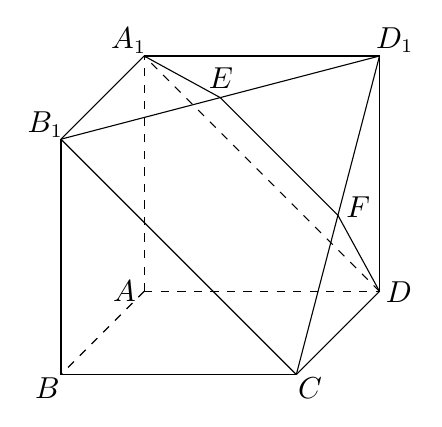
\begin{tikzpicture}[x=1pt, y=1pt,
    every node/.style={font=\fontsize{10.5pt}{12.6pt}\selectfont, inner sep=0pt}]
  % ---------- 实线 12 条（清单 §F04.2(a)）----------
  \begin{scope}[line width=0.3985pt]
    \draw (304.3280,364.6980) -- (331.8181,349.6667);   % P011 A₁E
    \draw (331.8181,349.6667) -- (374.3397,307.1451);   % P012 EF
    \draw (374.3397,307.1451) -- (389.3710,279.6550);   % P013 FD
    \draw (359.3083,249.5923) -- (389.3710,279.6550);   % P002 CD
    \draw (274.2653,249.5923) -- (359.3083,249.5923);   % P003 BC
    \draw (304.3280,364.6980) -- (274.2653,334.6353);   % P004 A₁B₁
    \draw (274.2653,334.6353) -- (389.3710,364.6980);   % P005 B₁D₁
    \draw (304.3280,364.6980) -- (389.3710,364.6980);   % P006 A₁D₁
    \draw (274.2653,249.5923) -- (274.2653,334.6353);   % P007 BB₁
    \draw (274.2653,334.6353) -- (359.3083,249.5923);   % P008 B₁C
    \draw (359.3083,249.5923) -- (389.3710,364.6980);   % P009 CD₁
    \draw (389.3710,279.6550) -- (389.3710,364.6980);   % P010 DD₁
  % ---------- 虚线 4 条（清单 §F04.2(b)）----------
    \draw[dash pattern=on 2.98883pt off 2.98883pt]
          (304.3280,279.6550) -- (389.3710,279.6550);   % P014 AD（被遮挡水平棱）
    \draw[dash pattern=on 2.98883pt off 2.98883pt]
          (389.3710,279.6550) -- (304.3280,364.6980);   % P015 DA₁（截面边）
    \draw[dash pattern=on 2.98883pt off 2.98883pt]
          (304.3280,279.6550) -- (274.2653,249.5923);   % P016 AB（被遮挡 45° 棱）
    \draw[dash pattern=on 2.98883pt off 2.98883pt]
          (304.3280,279.6550) -- (304.3280,364.6980);   % P017 AA₁（被遮挡竖直棱）
  \end{scope}
  % ---------- 字母标签（源墨迹实测中心）----------
  \node at (297.220,279.805) {$A$};    % L q19_A   清单 em 框 (297.471,278.184)
  \node at (269.329,244.611) {$B$};    % L q19_B   清单 em 框 (269.458,243.494)
  \node at (364.274,244.518) {$C$};    % L q19_C   清单 em 框 (363.835,243.494)
  \node at (396.314,279.533) {$D$};    % L q19_D   清单 em 框 (396.517,278.184)
  \node at (298.707,370.260) {$A_1$};  % L q19_A1  清单 em 框 (299.472,368.577)
  \node at (268.633,339.939) {$B_1$};  % L q19_B1  清单 em 框 (269.458,338.557)
  \node at (394.922,370.375) {$D_1$};  % L q19_D1  清单 em 框 (394.516,368.577)
  \node at (332.103,356.753) {$E$};    % L q19_E   清单 em 框 (331.486,355.568)
  \node at (381.685,310.000) {$F$};    % L q19_F   清单 em 框 (380.843,308.871)
\end{tikzpicture}
